%!TEX root = ../report.tex
%\cleardoublepage
%\clearpage
%
%\appendix
%\appendixpage
%\addappheadtotoc

\begin{appendices}
			
	%\addcontentsline{toc}{part}{\appendixname}
				
	\renewcommand{\thechapter}{\Alph{chapter}}
	\renewcommand{\thesection}{\thechapter.\arabic{section}}
	\renewcommand{\thesubsection}{\thesection.\arabic{subsection}}
	\renewcommand{\thesubsubsection}{\thesubsection.\arabic{subsubsection}}
	
	\chapter{Hardware Architecture}
	\section{Server Specification}
	% Probably move this into appendix
	\begin{table}[!htbp]
	    \centering
	    \begin{tabular}{L{\tw{0.2}} L{\tw{0.4}}}
	    \toprule
	    \multicolumn{2}{c}{Dell PowerEdge R530 Specification} \\ \midrule
	    \textbf{Item Description} & Dell PowerEdge R530 - E5-2620V3 Xeon 2.4 GHz - 16 GB - 1 TB \\
	    \textbf{Type} & Server - rack-mountable \\
	    \textbf{Height (Rack Units)} & 2U \\
	    \textbf{Processor} & 1 x Intel Xeon E5-2620V3 / 2.4 GHz (3.2 GHz) (6-core) \\
	    \textbf{Processor Main Features} & Intel Turbo Boost Technology 2 \\
	    \textbf{Cache Memory} & 15 MB \\
	    \textbf{Cache per processor} & 15 MB \\
	    \textbf{RAM} & 16 GB (installed) / 384 GB (max.) - DDR4 SDRAM - 2133 MHz \\
	    \textbf{Storage Controller} & RAID (SATA 6Gb / s) (Dell PERC H330) \\
	    \textbf{Optical Storage} & DVD burner \\
	    \textbf{Graphics Controller} & Matrox G200 \\
	    \textbf{Video Memory} & 16 MB \\
	    \textbf{Network} & GigE \\
	    \textbf{Dimensions} &  (WxDxH)48.24 cm x 64.6 cm x 8.68 cm \\
	    \textbf{Weight} & 2.14 kg \\
	    \bottomrule
	    \end{tabular}
	\caption{Hardware specification of Dell PowerEdge R530}
	\label{table:server-specs}
	\end{table}
	
	\chapter{Software Architecture}
	\section{Database diagram}
	\begin{figure}[H]
		\centering
		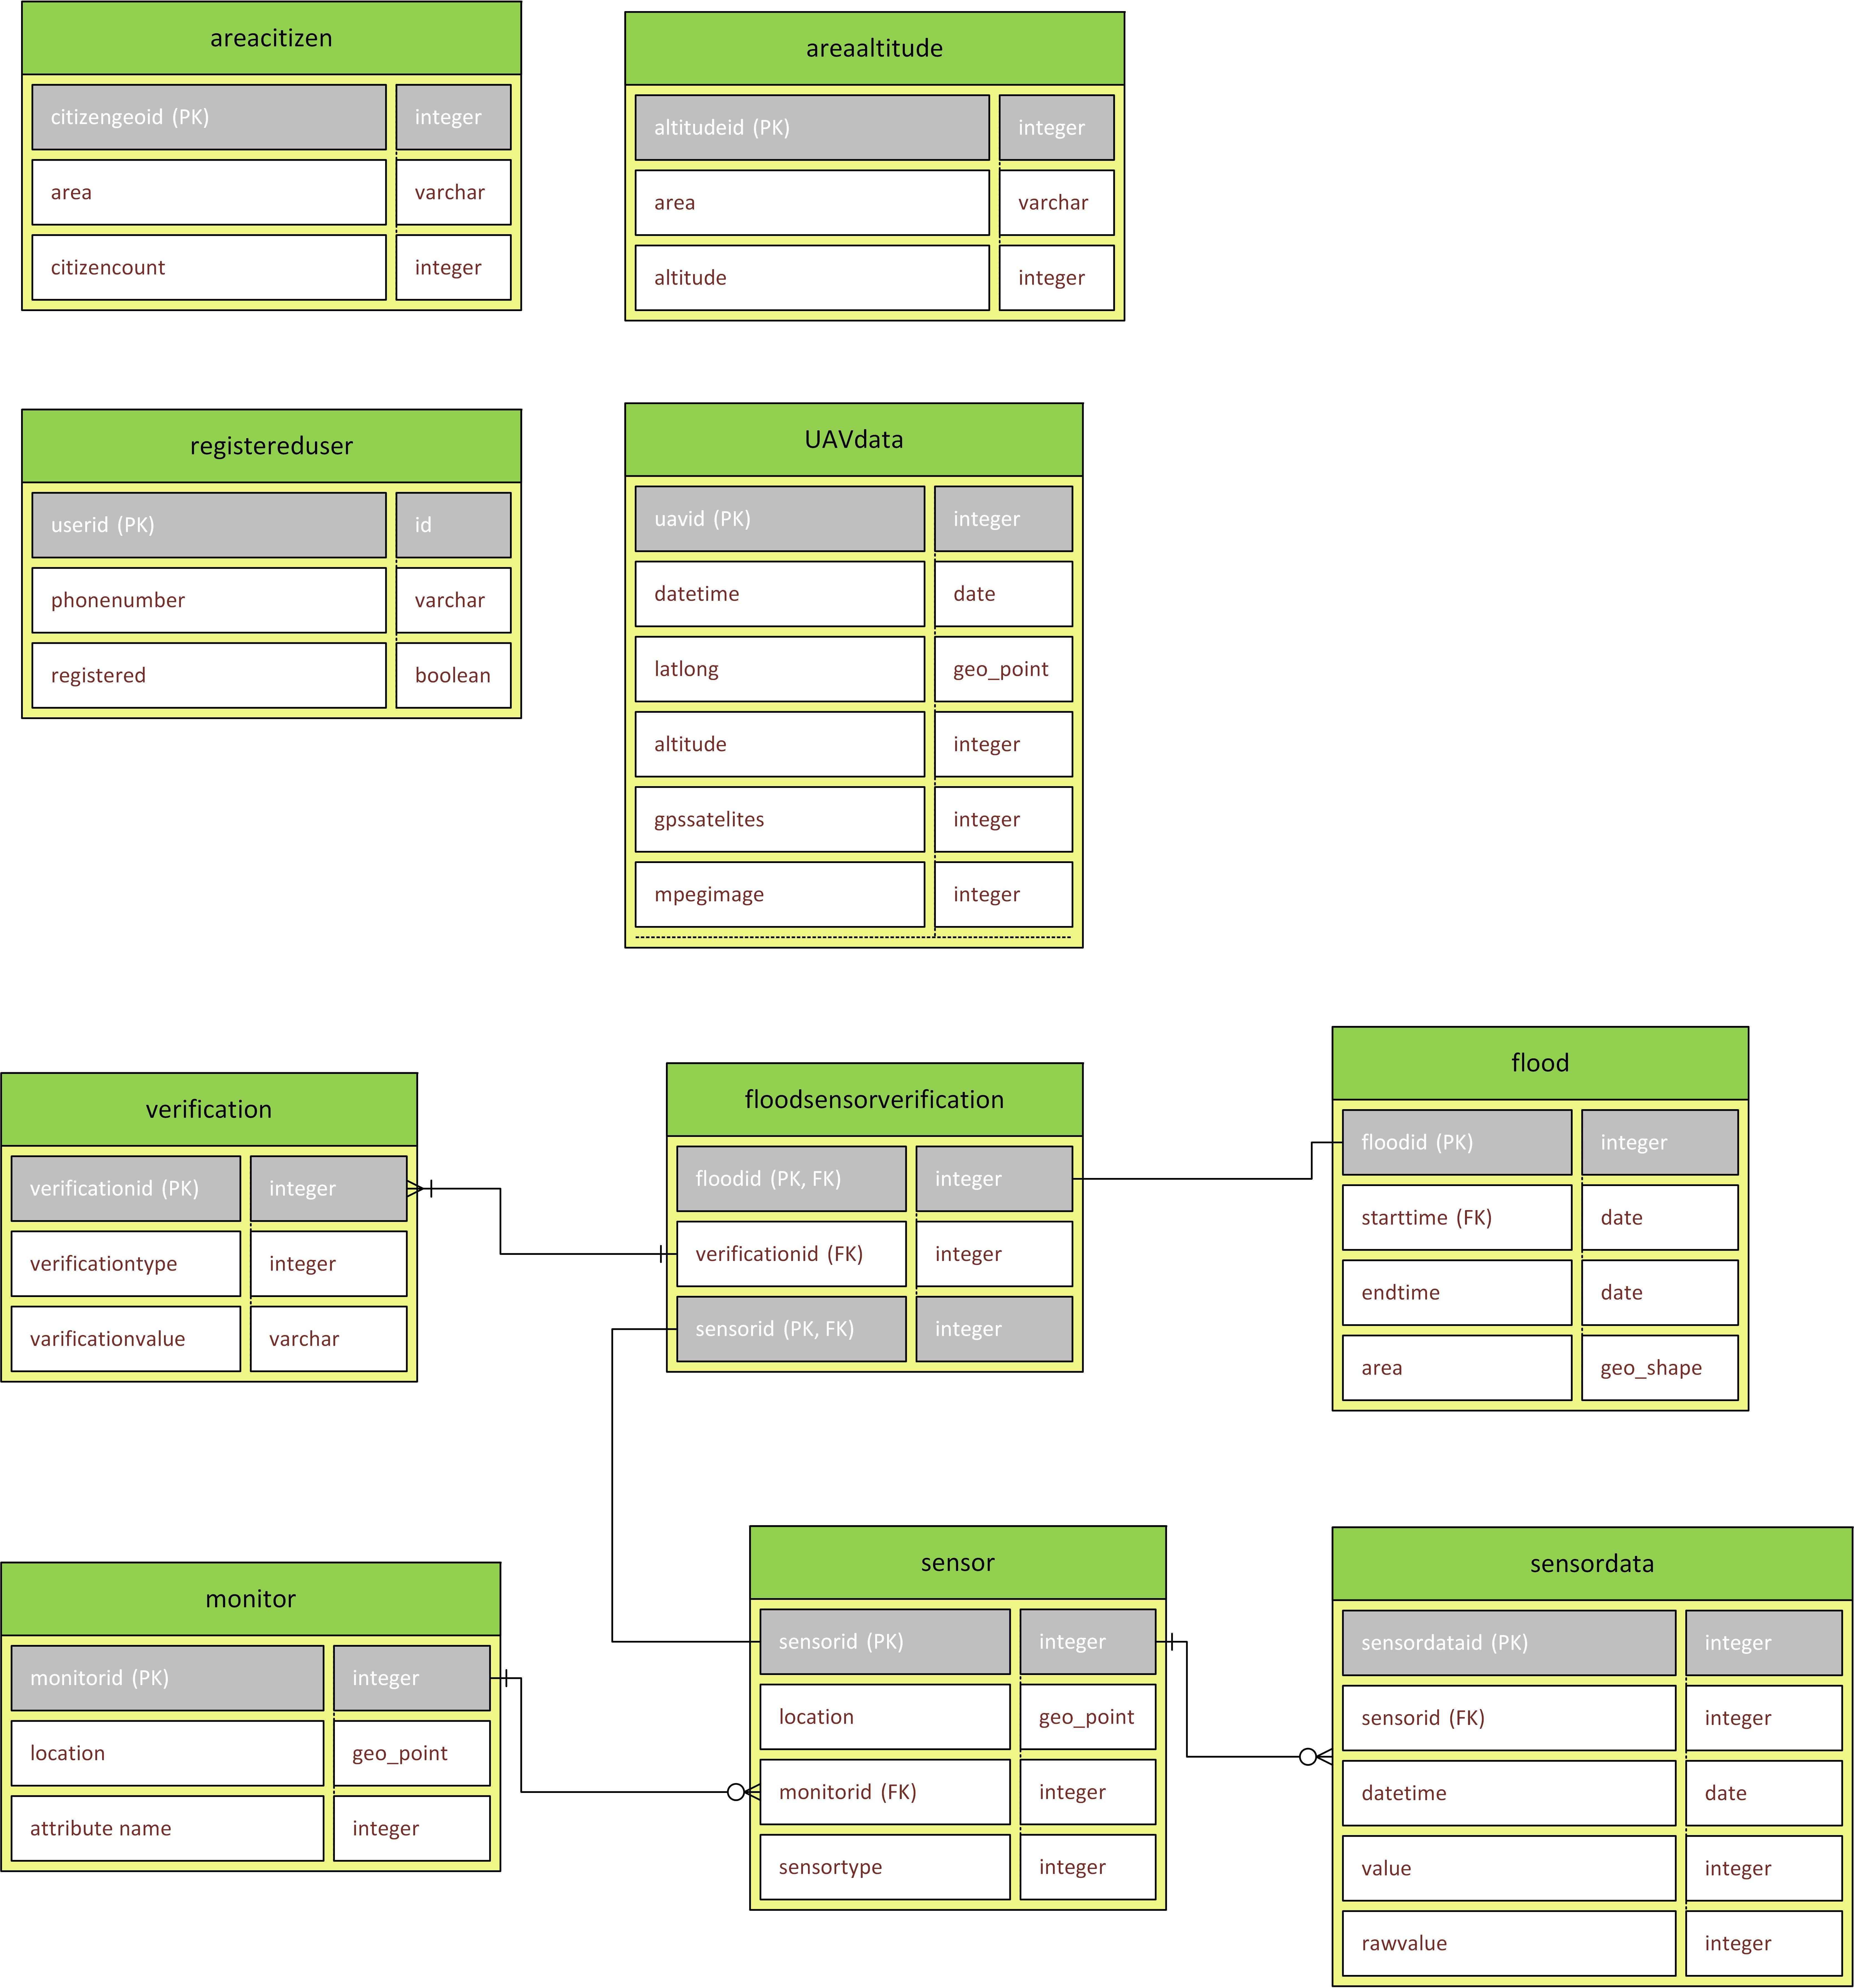
\includegraphics[height=14cm, width=0.9\textwidth]{{\viewimages/database}.jpg}
		\caption{Database diagram}
		\label{fig:database}
	\end{figure}

	% \afterpage{
	\begin{landscape}
	\section{Activity diagram}
	\begin{figure}[H]
		\centering
		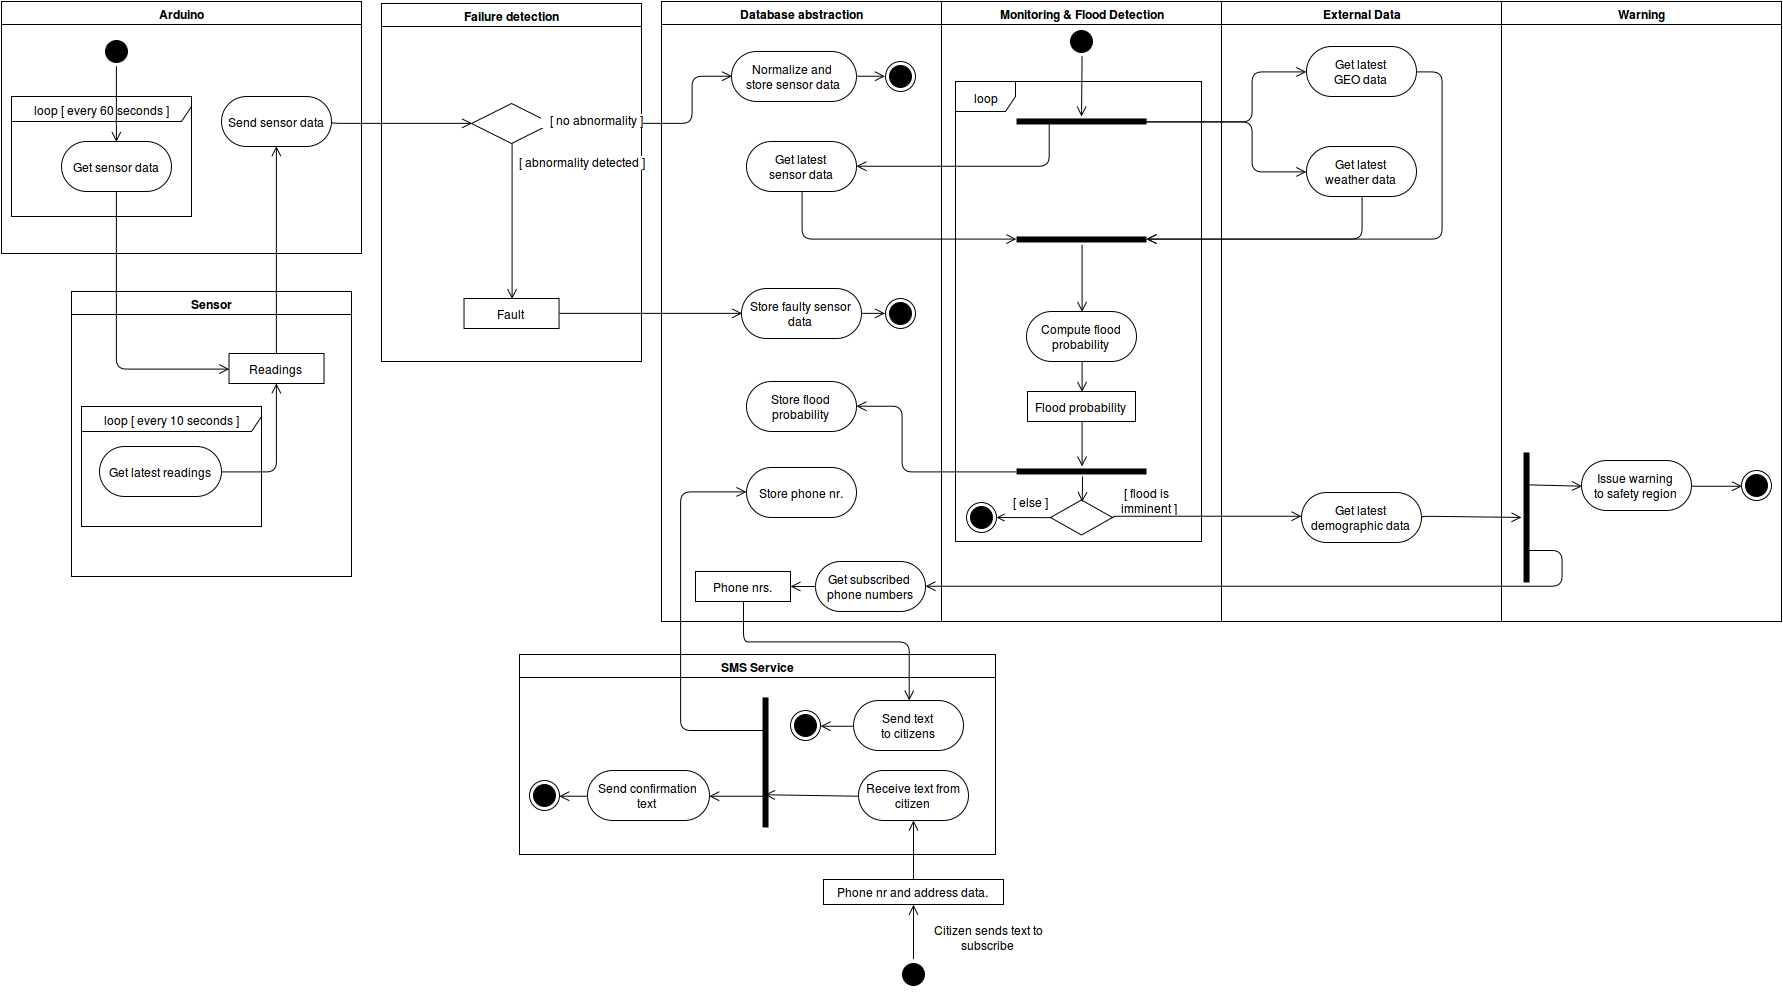
\includegraphics[keepaspectratio=true,width=1.0\textwidth]{{\viewimages/activity_monitoring}.png}
		\caption{An activity diagram of the flood monitoring process}
		\label{fig:activity-monitoring}
	\end{figure}
	% \end{landscape}
	% }
	
	% \afterpage{
	% \begin{landscape}
	\section{Deployment diagram}
	\begin{figure}[H]
		\centering
		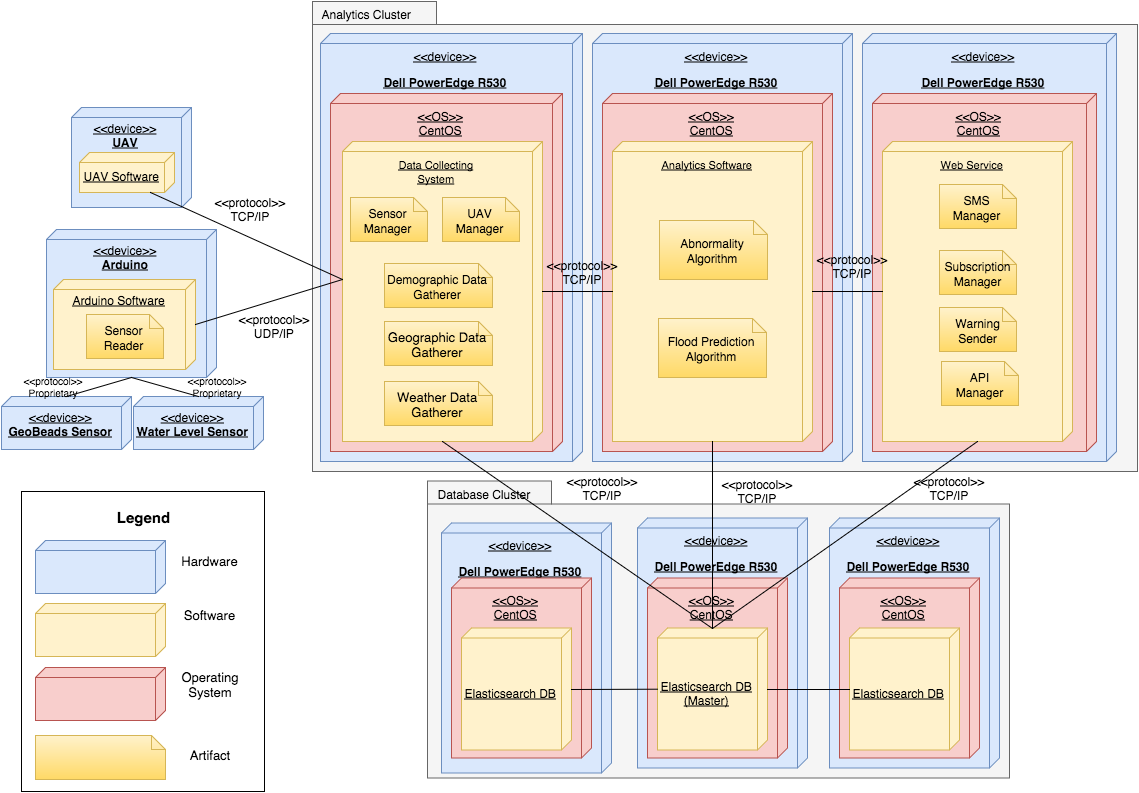
\includegraphics[keepaspectratio=true,width=0.8\textwidth]{{\viewimages/deployment-view}.png}
		\caption{Deployment diagram}
		\label{fig:deployment-diagram}
	\end{figure}
	\end{landscape}
	% }\clearpage

	%!TEX root = ../report.tex
\chapter{Time Tracking}
\label{App: Time Tracking}

%\section{Week #}
%\begin{tabular}{p{0.2\textwidth} p{0.7\textwidth} p{0.1\textwidth}}
%    \textbf{Person} & \textbf{Task} & \textbf{Hours} \\ \midrule
%	Eedema &  &  \\ \midrule
%	Putra &  &  \\ \midrule
%	Fakambi & & \\ \midrule
%	Schaefers &  & \\ \midrule
%	Brandsma &  & \\ \midrule
%	Menninga &  &  \\ \midrule
%\end{tabular}

\section{Week 1}
\begin{tabular}{L{0.2\textwidth} L{0.7\textwidth} L{0.1\textwidth}}
    \textbf{Person} & \textbf{Task} & \textbf{Hours} \\ \toprule
	Eedema & Reviewing the document, reading the assignment, initializing requirements, \& installing environment for project & 8 \\ \midrule
	Putra & Initial preparation for the course & 5 \\ \midrule
	Fakambi & Reading the document and assignment, Preparation and drafts with ideas & 5 \\ \midrule
	Schaefers & Setting up the working environment, create the context page and analysis page drafts. Setting up and improving the the document structure. & 8\\ \midrule
	Klinkenberg & & \\ \midrule
	Brandsma & Creating working environment, reading assignment, first draft business part & 8\\ \midrule
	Menninga & Reading assignment, setting up working environment, first non-functional requirements & 5 \\ \bottomrule
\end{tabular}

\section{Week 2}
\begin{tabular}{L{0.2\textwidth} L{0.7\textwidth} L{0.1\textwidth}}
    \textbf{Person} & \textbf{Task} & \textbf{Hours} \\ \toprule
	Eedema & Coaching session, project planning session and work on business information chapters & 9  \\ \midrule
	Putra & Coaching session, project planning session, project meeting, first version of stakeholder part of requirements & 7.5 \\ \midrule
	Fakambi & Coaching session , project meeting, work on Non functional requirements & 7 \\ \midrule
	Schaefers & First coaching session, improved and enhanced the context and business information chapters. Also created a quality attributes prioritization table.& 8 \\ \midrule
	Klinkenberg & Coaching session, meetings, providing feedback on requirements & 5.5\\ \midrule
	Brandsma & First version of use-cases, coaching session, meeting, use-cases, architectural vision & 6.5 \\ \midrule
	Menninga & First version of the functional requirements, coaching session, meeting & 10.25 \\ \bottomrule
\end{tabular}

\section{Week 3}
\begin{tabular}{p{0.2\textwidth} p{0.7\textwidth} p{0.1\textwidth}}
   \textbf{Person} & \textbf{Task} & \textbf{Hours} \\ \midrule
	Eedema &  Coaching, meetings, analysis, business part, reviewing & 14  \\ \midrule
	Putra & Coaching session, meetings, proofread on chapter 1 and 2, revising stakeholders, database decision part of analysis, and preparing \LaTeX{} file for the presentation & 10 \\ \midrule
	Fakambi & Coaching session, meetings, Non functional requirements and Risk assessment & 10.5\\ \midrule
	Schaefers & Coaching session, meetings, reviewing, Business section & 12 \\ \midrule
	Klinkenberg & Coaching session, meetings, technical requirements, analysis, reviewing & 13.5 \\ \midrule
	Brandsma & Coaching session, meeting, architectural vision, use-cases, analysis & 9 \\ \midrule
	Menninga & Coaching session, meetings, updates functional requirements, reviewing entire document, updated assumptions and some improvements to structure of analysis, added decision about type of water level sensor. & 14.0 \\ \midrule
\end{tabular}

\section{Week 4}
\begin{tabular}{p{0.2\textwidth} p{0.7\textwidth} p{0.1\textwidth}}
   \textbf{Person} & \textbf{Task} & \textbf{Hours} \\ \midrule
	Eedema & Coaching session, meetings, business chapter, review 3, presentations, peer review &13  \\ \midrule
	Putra & Coaching session, meetings, presentation prep., improving business rationale, review chapter 2, making draft of chapter 5, 6, and 7 & 14 \\ \midrule
	Fakambi & Coaching session , meetings , Work on and improvements chapter 3.5 to 3.8 & 12 \\ \midrule
	Schaefers & Researched on sensors and other EWS's. Then created the system architecture model diagram and vision diagram for the presentation I had to present in. Created/improved other diagrams. Researched about the costs of these kinds of systems and created/enhanced the business cost section. & 20 \\ \midrule
	Brandsma & Coaching session, meetings , reviewing group 1, architectural vision, use-cases, reviewing, improving chapter 4 & 16.5\\ \midrule
	Menninga & Coaching session, presentation prep., meeting, improvements FR and risks, review ch. 4, improvements to NFR and Risk Assessment & 14.0 \\ \midrule
\end{tabular}

\section{Week 5}
\begin{tabular}{p{0.2\textwidth} p{0.7\textwidth} p{0.1\textwidth}}
    \textbf{Person} & \textbf{Task} & \textbf{Hours} \\ \midrule
	Eedema & Coaching meetings, reviewing, chpt 5  & 13 \\ \midrule
	Putra & Coaching session, meetings, reviewing, working on initial work on chapter hardware, researching on servers, and working on server selection  & 15 \\ \midrule
	Fakambi & Coaching session, meetings, Work on chapter 6 Hardware architecture, drafts, design decision about UAVs & 12.0 \\ \midrule
	Schaefers & Created initial layer diagram, component diagram, sequense diagram and database design diagram. Researched and explained what new database to use.  & 15\\ \midrule
	Brandsma & Coaching session, meetings, chapter 5  & 13 \\ \midrule
	Menninga & Coaching session, meeting Tuesday, lots of improvements to chapter 3, expanding chapter 6 & 15.5 \\ \midrule
\end{tabular}

\section{Week 6}
\begin{tabular}{p{0.2\textwidth} p{0.7\textwidth} p{0.1\textwidth}}
    \textbf{Person} & \textbf{Task} & \textbf{Hours} \\ \midrule
	Eedema & Coaching, meetings, review, system overview, evaluation & 15 \\ \midrule
	Putra & Coaching session, meetings, reviews, hardware overview, deployment view & 13 \\ \midrule
	Fakambi & Coaching session, meetings, Work on chapter 6 Hardware architecture, drafts, design decision about UAVs, draft about chapter 7 & 9 \\ \midrule
	Schaefers & Meetings. Worked on the implementation and logical section of the software chapter. & 13 \\ \midrule
	Brandsma & &  \\ \midrule
	Menninga & Coaching session, meetings, reviews, hardware overview (sensors)/costs, implementation view, process view & 13.0 \\
	\midrule
\end{tabular}
	% %!TEX root = ../report.tex
\chapter{Todo} % (fold)
\label{sec:todo}
\todo[inline]{Create figure with processflow and place it somewhere logical}
% section todo (end)
\end{appendices}